% Options for packages loaded elsewhere
\PassOptionsToPackage{unicode}{hyperref}
\PassOptionsToPackage{hyphens}{url}
%
\documentclass[UTF8
]{ctexart}
\usepackage{lmodern}
\usepackage{amsmath}
\usepackage{amssymb}
\usepackage{graphicx}
\usepackage{ifxetex,ifluatex}
\ifnum 0\ifxetex 1\fi\ifluatex 1\fi=0 % if pdftex
  \usepackage[T1]{fontenc}
  \usepackage[utf8]{inputenc}
  \usepackage{textcomp} % provide euro and other symbols
\else % if luatex or xetex
  \usepackage{unicode-math}
  \defaultfontfeatures{Scale=MatchLowercase}
  \defaultfontfeatures[\rmfamily]{Ligatures=TeX,Scale=1}
\fi
% Use upquote if available, for straight quotes in verbatim environments
\IfFileExists{upquote.sty}{\usepackage{upquote}}{}
\IfFileExists{microtype.sty}{% use microtype if available
  \usepackage[]{microtype}
  \UseMicrotypeSet[protrusion]{basicmath} % disable protrusion for tt fonts
}{}
\makeatletter
\@ifundefined{KOMAClassName}{% if non-KOMA class
  \IfFileExists{parskip.sty}{%
    \usepackage{parskip}
  }{% else
    \setlength{\parindent}{0pt}
    \setlength{\parskip}{6pt plus 2pt minus 1pt}}
}{% if KOMA class
  \KOMAoptions{parskip=half}}
\makeatother
\usepackage{xcolor}
\IfFileExists{xurl.sty}{\usepackage{xurl}}{} % add URL line breaks if available
\IfFileExists{bookmark.sty}{\usepackage{bookmark}}{\usepackage{hyperref}}
\hypersetup{
  hidelinks,
  pdfcreator={LaTeX via pandoc}}
\urlstyle{same} % disable monospaced font for URLs
\usepackage{longtable,booktabs}
% Correct order of tables after \paragraph or \subparagraph
\usepackage{etoolbox}
\makeatletter
\patchcmd\longtable{\par}{\if@noskipsec\mbox{}\fi\par}{}{}
\makeatother
% Allow footnotes in longtable head/foot
\IfFileExists{footnotehyper.sty}{\usepackage{footnotehyper}}{\usepackage{footnote}}
\makesavenoteenv{longtable}
\setlength{\emergencystretch}{3em} % prevent overfull lines
\providecommand{\tightlist}{%
  \setlength{\itemsep}{0pt}\setlength{\parskip}{0pt}}
\setcounter{secnumdepth}{-\maxdimen} % remove section numbering

\date{}


\begin{document}

\hypertarget{header-n0}{%
\section{Google PageRank数学模型分析}\label{header-n0}}

\hypertarget{header-n2}{%
\subsection{摘要}\label{header-n2}}

小组希望通过介绍一个成功并广泛使用的数学模型------Google公司的Page
Rank算法,并解析该数学模型的原理。该数学模型使用了图论,概率统计,马尔可夫链等数学工具解释了在Google搜索中网页出现的次序是如何产生的。

PageRank算法的核心思想是

\begin{enumerate}
\def\labelenumi{\arabic{enumi}.}
\item
  如果一个网页被很多其他网页链接,说明这个网页具有很大参考性
\item
  如果一个具有很大参考性的网页有链接指向的其他网页,那么被链接到的网页也同样具有较大的参考系。
\end{enumerate}

\hypertarget{header-n9}{
\subsection{模型背景}\label{header-n9}}

Google出现以前实际上就有很多通用的或者专业领域的搜索引擎,但这个搜索引擎巨无霸最终能击败其他竞争对手,很大的原因是因为其使用了PageRank算法重新对搜索结果按重要性排序。Web页面检索数量巨大,所以一个检索的结果条目数量非常多。用户不可能从如此众多的结果中一一查找对自己有用的信息。所以,一个好的搜索引擎需要想尽办法将质量较高相关度更准确的页面排到前面。

如果单纯使用关键词占比评价页面重要性,每个页面发布者为了使自己的排名更好,可以这么做:在页面中加入一个隐藏的html元素比如一个div,其内容是某个相关关键词并重复一万次。这样,搜索引擎在计算该关键词的搜索结果时,其关键词占比就会非常高,从而做到排名靠前的效果。这种行为叫做“Term Spam”。早期搜索引擎深受这种作弊方法的困扰,加之基于关键词的评价算法本身也不甚合理,因此经常是搜出一堆质量低下的结果,用户体验大大打了折扣。

\hypertarget{header-n10}{%
\subsection{模型介绍}\label{header-n10}}

佩奇排名(PageRank),又称网页排名,是Google公司所使用的对其搜索引擎搜索结果中的网页进行排名的一种算法。

佩奇排名本质上是一种以网页之间的超链接个数和质量作为主要因素粗略地分析网页的重要性的算法。其基本假设是:更重要的页面往往更多地被其他页面引用。
其将从A页面到B页面的链接比作``A页面给B页面投票'',并根据投票来源(甚至来源的来源,即链接到A页面的页面)和投票对象的等级来决定被投票页面的等级。简述之就是一个高等级的页面可以提升其他低等级的页面。

算法由谷歌公司创始人之一的拉里·佩奇(Larry
Page)的名字來命名。谷歌搜索引擎用它来分析网页的相关性和重要性,在搜索引擎优化中經常被用來作为評估網頁优化的成效因素之一。目前为止,佩奇排名算法不再是谷歌公司用来给网页进行排名的唯一算法,但它是最早的,也是最著名的算法。

\hypertarget{header-n16}{%
\subsection{模型假设}\label{header-n16}}
我们将互联网想象成一个流网络,网络的节点就是一个个网页,如果两个网页见存在超链接的关系,那么他们之间就存在一条有向的连边。
PageRank算法假设输出概率分布能体现某位用户随机点击某个链接的概率。设定一个PR值,其物理意义为一个网页被访问的概率。PR值可以在任何规模文件计算得出,每个链接都指向该集合中的某个特定文件。PR值在区间(0,1),表示事件发生的概率。

\begin{figure}[htbp]
	\centering
	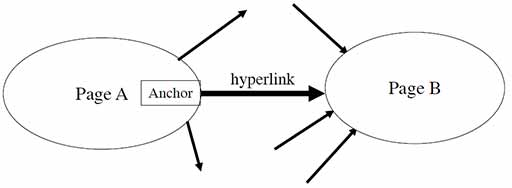
\includegraphics[width=3.2in]{1_1.jpg}
	\caption{基本模型}
	\label{img1}
\end{figure}

\hypertarget{header-n19}{%
\subsection{符号说明}\label{header-n19}}

\begin{longtable}[]{@{}ll@{}}
\toprule
符号 & 解释\tabularnewline
\midrule
\endhead
\(PR(x)\) & 表示页面x的PR值\tabularnewline
\(L(x)\) & 页面\(x\)链出的数量\tabularnewline
\(In(x)\) & 链入\(x\)页面的集合\tabularnewline
\(N\) & 集合中所有页面的数量\tabularnewline
\(d\) & 阻尼系数,又称修正值\tabularnewline
\(\gamma (x,y) \) & 从页面\(x\)指向页面\(y\)的链接数 与
页面\(y\)中含有外部链接总数 的比值\tabularnewline
\emph{M} & 表示页面之间出入概率的矩阵\tabularnewline
\bottomrule
\end{longtable}

\hypertarget{header-n46}{%
\subsection{模型建立}\label{header-n46}}

\hypertarget{header-n47}{%
\subsubsection{模型一}\label{header-n47}}

模型A假设有4个网页组成的集合即A,B,C,D四个页面,同一个页面中多个指向相同的链接视为同一个链接,每个页面初始的PR值相同为1。

情况1:当所有页面都只链接至A,如下图2
\begin{figure}[htbp]
	\centering
	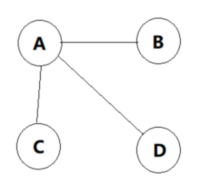
\includegraphics[width=2.2in]{1_2.png}
	\caption{情況1}
	\label{img2}
\end{figure}

那么\(PR(A)\)就为\(B,C,D\)的\(PR\)值之和,即

\[PR(A)=PR(B)+PR(C)+PR(D)\]

情况2:当所有的页面都如下图链接,即B链接倒A和C,C链接倒A,D链接倒A,B,C。

\[PR(A)= {PR(B)\over 2}+{PR(C)\over 1}+{PR(D)\over 3}\]

换成j加上修正系数可以变成更通用的形式,当遇上没有外链接的页面,传递出去的PR值为0,如情况1的A页面,会递归地导致指向它的页面PR值得计算结果同样为零。所以对每个页面的PR值,赋一个最小值\$(1-d)/
N

\[PR(A)=  \Bigl({PR(B)\over L(B)}+{PR(C)\over L(C)}+{PR(D)\over L(D)}+\cdots\bigr)\times d+{1-d\over N}\]

从上述公式看出,一个页面的PR值取决于指向其的其他页面。

\hypertarget{header-n57}{%
\subsubsection{模型二}\label{header-n57}}

对于修正系数的理解,我们也可以假设某人在浏览器随机打开某些页面并点击了某些链接,并不断点击网页上的链接直到进入一个没有外部链接的网页,那此时他会随机浏览其他的网页。为了方便计算,上述公式又可以转化成如下公式:

\[PR(p_i)=d\times \sum_{p_j \in In(p_i)}{PR(p_j)\over L(p_j)}+{1-d\over N}\]

所有页面 的PR值可以用向量的形式表示,特征向量为

\[R=\begin{pmatrix}
PR(p_1)\\PR(p_2)\\PR(p_3)\\\vdots\\PR(p_N)
\end{pmatrix}\]

使用\(\gamma(x,y)\)代替原模型链接某个页面x的全职之和

\[\gamma(x,y)={1\over L(y)}\]
\[when x=y,\gamma(x,y)=0\]

于是我们联系线性代数中的矩阵方法,总结出以下求解公式

\[R=\begin{pmatrix}{1-d\over N}\\{1-d\over N}\\\vdots\\{1-d\over N }\end{pmatrix}+d
\begin{pmatrix}\gamma(p_1,p_1)&\gamma(p_1,p_2)&\cdots&\gamma(p_1,p_n)
\\\gamma(p_2,p_1)&\gamma(p_2,p_2)&\cdots&\gamma(p_2,p_n)
\\\vdots&\vdots&\ddots&\vdots
\\\gamma(p_n,p_1)&\gamma(p_n,p_2)&\cdots&r(p_n,p_n)
\end{pmatrix}R\]

由于上述修改后的邻接矩阵的巨大的特征值,所以几次迭代后即可在极高的精确度下估计PageRank特征向量R的值。可以得出由于\(d<0\),上述求解公式为收敛的马尔可夫链。

\hypertarget{header-n68}{%
\subsection{模型验证}\label{header-n68}}

依然以图一作为例子,此时使用继续使用矩阵\(M\)表示页面之间出入的关系

\[M=\begin{pmatrix}\gamma(p_1,p_1)&\gamma(p_1,p_2)&\cdots&\gamma(p_1,p_n)
\\\gamma(p_2,p_1)&\gamma(p_2,p_2)&\cdots&\gamma(p_2,p_n)
\\\vdots&\vdots&\ddots&\vdots
\\\gamma(p_n,p_1)&\gamma(p_n,p_2)&\cdots&r(p_n,p_n)
\end{pmatrix}=\begin{pmatrix}0&1/2&0&0\\
1/3&0&0&1/2\\
1/3&0&1&1/2\\
1/3&1/2&0&0
\end{pmatrix}\]

设 \emph{e} 为分量全部为1的列向量,定义矩阵 \emph{A}:

\[A=dM+{(1-d)\over N}ee^T\]
\[\Rightarrow R_{n+1}=AR_n\]

由于这个马尔可夫过程收敛,且有\(\lim_{n \rightarrow \infty}R_{n}\)存在,与初始值\(R_0\)的选取无关,由于状态转移矩阵A满足

\begin{enumerate}
\def\labelenumi{\arabic{enumi}.}
\item
  A为随机矩阵,因为\(\forall_{i=1...n} \sum_{j=1}^{n}A_{ij}=1 \)
\item
  A为不可约矩阵
  ,因为A对应的有向图是强连通的。其中无链接通入的网页也有概率通过输入网址进行访问。
\item
  A为非周期矩阵
\end{enumerate}

由上面三个原因证明了PageRank算法的正确性。

\hypertarget{header-n83}{%
\subsection{模型PR值计算方法}\label{header-n83}}

\hypertarget{header-n84}{%
\subsubsection{幂迭代法}\label{header-n84}}
给定\(n\times n\)的网页链接矩阵\(M\)
首先给每个页面赋予随机的PR值,然后通过\(R_{n+1}=AR_{n}\)不断地迭代PR值。当满足下面的不等式后迭代结束,获得所有页面的PR值:

\[|P_{n+1}-P_n|<\lambda\]

\hypertarget{header-n87}{%
\subsubsection{特征值法}\label{header-n87}}

当马尔可夫链收敛的时候,必有若\(P=AP\),
则P为矩阵A特征值1对应的特征向量

\hypertarget{header-n90}{%
\subsubsection{代数法}\label{header-n90}}

相似的,当马尔可夫链收敛时,必有

\[ R = A R \\
\Rightarrow R = \Bigl( d M + \frac{(1 - d)}{N}ee^T \Bigr) R \]
因为e为所有分量都为 1 的列向量,R的所有分量之和为1,所以
\[ R = d MR + \frac{(1 - d)}{N}e \]
\[\Rightarrow (ee^T - d M)R = \frac{(1 - \alpha)}{N}e \]
\[\Rightarrow R = (ee^T - d M)^{-1} \frac{(1-d)}{N}e \]

\hypertarget{header-n85}{%
\subsection{Spider Traps现象与平滑处理}\label{header-n85}}
如果把真实的网页集合成转移矩阵,那么这将是一个极为稀疏的矩阵。从矩阵论知识可以推断,极度稀疏的转移矩阵迭代相乘可能会使得向量v变得非常不平滑\footnote{平滑,又叫做平滑过程,是统计学和图像处理中的概念。意思是把在训练样本中出现过的事件的概率适当减小,把减小得到的概率密度分配给训练语料中没有出现过的事件,这个过程有时也称为减值},即一些节点拥有很大的PR值,而其他大多数节点PR值接近0。而一种叫做Spider Traps节点的存在加剧了这种不平滑。如图3
\begin{figure}[htbp]
	\centering
	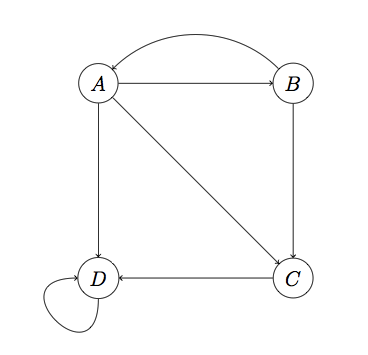
\includegraphics[width=3.2in]{1_3.png}
	\caption{Spider Traps现象图}
	\label{img2}
\end{figure}
如图三,结点D有外链不是自反孤立点,但是它链接只指向自己。这种节点叫做Spider Trap。如果对这个图按照上述公式进行计算,会发现结点D的PR值会越来越大趋近于1,而其它节点A,B,C的PR值几乎归零。

为了解决由于矩阵稀疏性和Spider Traps带来的问题,Google对PageRank计算方法进行一个平滑处理,具体做法是在模型二用户会随机打开某个页面的指向其他页面链接基础上,继续假设任何一个页面浏览的用户都有可能以一个极小的概率瞬间转移到另外一个随机页面\footnote{又叫心灵转移(teleporting),意为在浏览该页面时可能会随机跳转到一个无关系的页面}。当然,这两个页面可能不存在链接,因此不可能真的直接转移过去,只是为了算法需要而强加的一种纯数学意义的概率数字。通过如此平滑处理之后,新的公式为
\[ {R}'=(1-d)MR+e\frac{d}{N}\]
其中修正值d往往被设置为一个比较小的参数(0.2或者更小的值),e为N维单位向量,加入e的原因是这个公式的前半部分是向量,因此必须将d/N转为向量才能相加。这样,整个迭代的计算过程就变得平滑,因为每次迭代的结果除了依赖原本的转移矩阵M外,还依赖一个小概率的随机页面转移。以图三为例,根据图可得转移矩阵M如下
\[ M=\begin{bmatrix} 0 & 1/2 & 0 & 0\\ 1/3 & 0 & 0 & 0\\ 1/3 & 1/2 & 0 & 0\\ 1/3 & 0 & 1 & 1 \end{bmatrix}\]
假设修正值d为0.2,加权之后的转移矩阵如下
\[M=\begin{bmatrix} 0 & 2/5 & 0 & 0\\ 4/15 & 0 & 0 & 0\\ 4/15 & 2/5 & 0 & 0\\ 4/15 & 0 & 4/5 & 4/5 \end{bmatrix}\]
最后平滑稀疏矩阵之后的结果为
\[{R}'=\begin{bmatrix} 0 & 2/5 & 0 & 0\\ 4/15 & 0 & 0 & 0\\ 4/15 & 2/5 & 0 & 0\\ 4/15 & 0 & 4/5 & 4/5 \end{bmatrix}v+\begin{bmatrix} 1/20\\ 1/20\\ 1/20\\ 1/20 \end{bmatrix}\]
按照这个公式继续迭代,发现很多原来的Spider Traps效应被很好的控制住了,一定概率上确保了页面有比较合理的PR值。


\hypertarget{header-n94}{%
\subsection{模型缺陷}\label{header-n94}}
PageRank模型的缺陷在于旧的页面PR值往往比新的页面要高。由于新页面创建时间不长,只会有很少链接指向新页面导致PR值不高。同时,由于较低的PR值,新页面在Google的搜索结果中排名靠后,导致一个恶性循环:新页面因为PR值低很难受到浏览者关注,同时又需要更多的浏览者进入并分享提高该页面的PR值。
模型还缺乏了对主题特征的分类, 如模型无法分辨用户输入的苹果是Apple公司还是苹果这个食物。
此后,Google公司在搜索结果排名中也使用了其他的模型为网页排名作出改善,在搜索结果中增加了主题分类。

\hypertarget{header-n95}{%
\subsection{使用MapReduce技术进行模拟的}\label{header-n95}}
我们在模拟的时候使用上面的演算过程,采用矩阵相乘,不断迭代,直到迭代前后概率分布向量的值变化不大,一般迭代到30次以上就收敛了。现实生活中的网页结构的转移矩阵非常大,目前的网页数量已经超过100亿,所以转移矩阵是100亿*100亿的矩阵,直接按矩阵乘法的计算方法不可行,需要借助Map-Reduce的计算方式来解决。实际上,Google发明Map-Reduce最初就是为了分布式计算大规模网页的PageRank,Map-Reduce的PageRank有很多实现方式,论文将介绍最简单的类型。

考虑转移矩阵是一个很多的稀疏矩阵,我们可以用稀疏矩阵的形式表示,我们把web图中的每一个网页及其链出的网页作为一行,这样第四节中的web图结构用如下方式表示:
\begin{figure}[htbp]
	\centering
	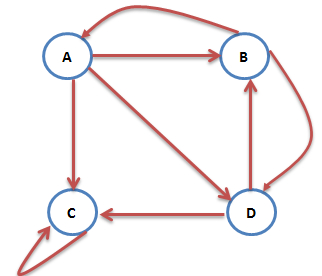
\includegraphics[width=3.2in]{1_4.jpg}
	\caption{MapReduce例子}
	\label{img4}
\end{figure}
\[A \to B,C,D\]
\[B \to A,D\]
\[C \to C\]
\[D \to B,C\]
A有三条出链,分别指向B、C、D,实际上,我们爬取的网页结构数据就是这样的。

\hypertarget{header-n100}{
\subsubsection{Map阶段}
\label{header-n100}}

Map操作的每一行,对所有出链发射当前网页概率值的\(1/k\),\(k\)是当前网页的链接链出数,以A结点为例子,Map输出\[<B,1/3*1/4>,<C,1/3*1/4>,<D,1/3*1/4>\];

\hypertarget{header-n101}{
	\subsubsection{Reduce阶段}
	\label{header-n101}}

Reduce操作收集网页id相同的值,累加并按权重计算,pj=a*(p1+p2+...Pm)+(1-a)*1/n,其中m是指向网页j的网页j数,n所有网页数。

思路就是这么简单,但是实践的时候,怎样在Map阶段知道当前行网页的概率值,需要一个单独的文件专门保存上一轮的概率分布值,先进行一次排序,让出链的矩阵行与概率值按网页id出现在同一Mapper里面,整个流程如图5

\begin{figure}[htbp]
	\centering
	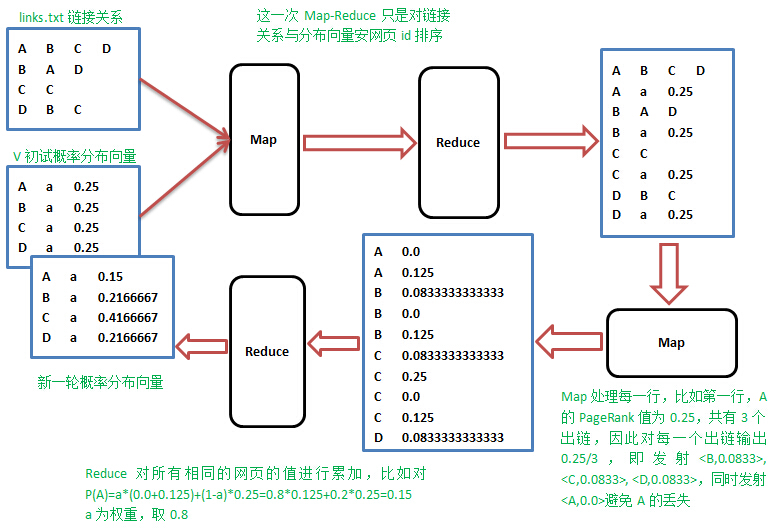
\includegraphics[width=5.6in]{1_5.jpg}
	\caption{MapReduce过程}
	\label{img5}
\end{figure}
这就是基本的MapReduce实现.

\pagebreak

\hypertarget{header-n97}{%
\subsection{总结}\label{header-n97}}
通过研究分析Google的PageRank算法,我们理解了一个简单的线性代数和矩阵模型在计算机科学中的应用。后人将PageRank算法称作“天才”般的算法。Google在当时背景下提出该算法,并申请了专利保护。此举充分保护了当时弱小的Google公司,并使得Google一举成为全球首屈一指的搜索引擎。作为软件学院的学生,我们通过分析研究PageRank算法,认识到了数学模型以及算法在互联网企业发展中的重要性。



\hypertarget{header-n98}{
\subsection{参考文献}\label{header-n98}}
[1] Page, Lawrence, et al. The PageRank citation ranking: Bringing order to the web. Stanford InfoLab, 1999.

[2] CodeMeals,PageRank算法简介及Map-Reduce实现\\
 https://www.cnblogs.com/fengfenggirl/p/pagerank-introduction.html

[3] S. Brin and L. Page, “Anatomy of a large-scale hypertextual web search engine,” Proc. 7th Intl. World-Wide-Web Conference, pp. 107–117, 1998.


\end{document}
